‌\section{Introducción}
Con este diseño se busca un sistema de venta de telefonía celular que permita tener un alto grado de confiabilidad tanto para el vendedor como para el cliente, que mantenga interconectadas a las distintas partes de la empresa (marketing - ventas - facturación - stock) en todo momento, que automatice algunos procesos internos de la empresa y que agilice y mejore el rendimiento de ventas.\\

\section{Diagrama de Contexto}

\begin{figure}[h!]
  \centering
  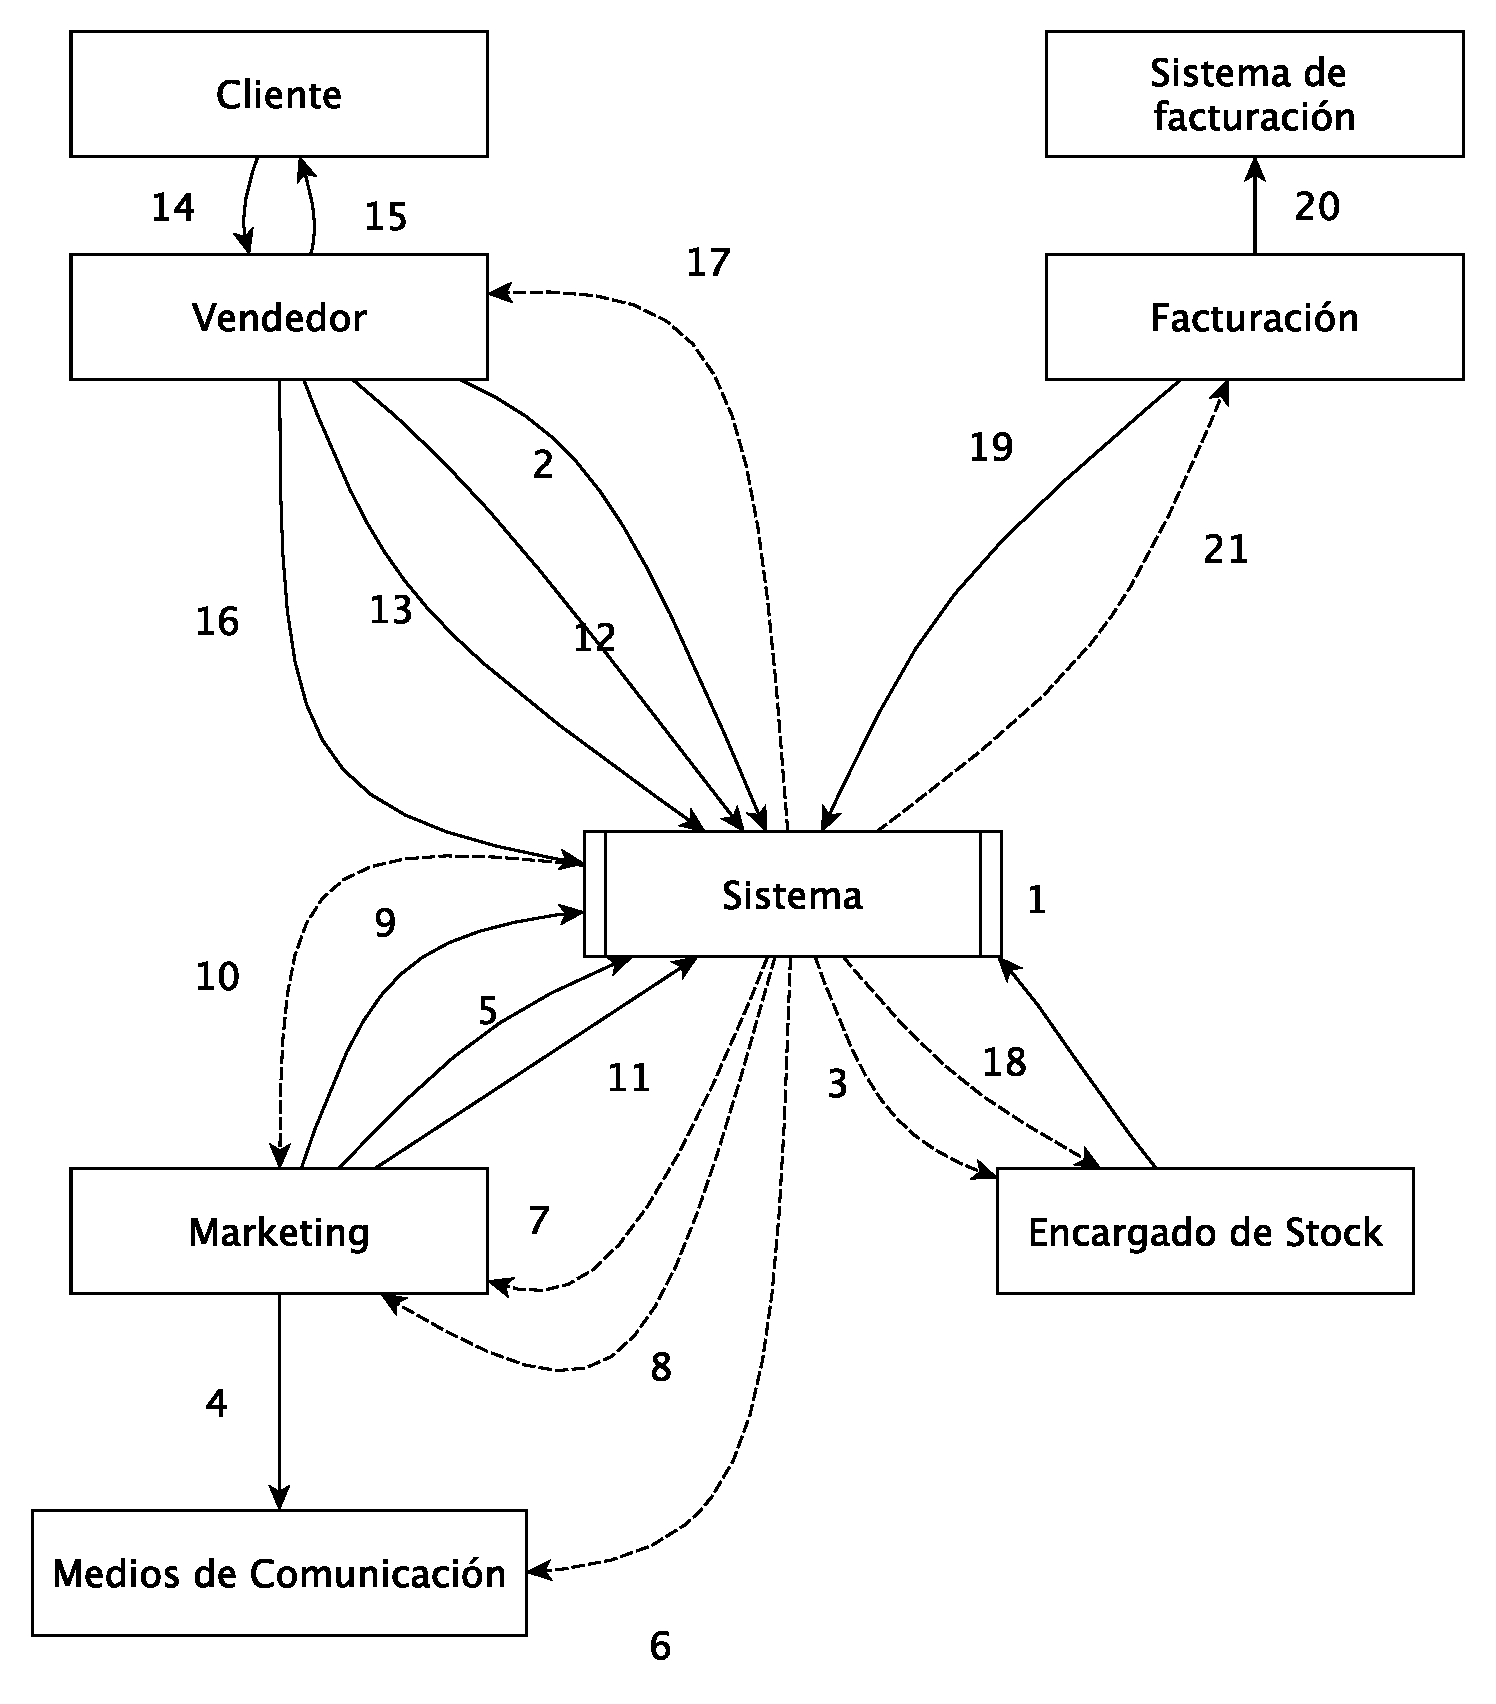
\includegraphics[width=0.5\textwidth]{./imagenes/contexto_1.pdf}
  \caption{Diagrama de Contexto para Sistema de Venta de Celulares}
\end{figure}

\subsection{Eventos}

\begin{enumerate}

  \item Ingresar nuevos equipos.
  \item Registrar o cancelar reserva de equipos.
  \item Notificar la confirmación de reserva de equipos.
  \item Monitorear los medios tradicionales de comunicación.
  \item Seleccionar usuarios y sitos a monitorear.
  \item Monitorear competencia por internet.
  \item Enviar informe de estado del mercado.
  \item Notificar que se creó promoción automáticamente. (vale para mercacdo y stock acumulado)
  \item Validar promoción creada automátiacmente. (vale para mercacdo y stock acumulado)
  \item Notificar stock acumulado.
  \item Dar Alta o baja nueva promoción.
  \item Consultar en el momento datos del cliente.
  \item Consultar en el momento promociónes para el cliente.
  \item Comunicar necesidades.
  \item Convencer de adquirir promoción.
  \item Seleccionar la promoción adquirida por el cliente.
  \item Confirmar o rechazar promoción por disponibilidad de stock.
  \item Alertar cuando stock está pronto a acabarse.
  \item Confirmar o rechazar venta.
  \item Cargar la venta de los equipos y las líneas.
  \item Notificar venta nueva para ser verificada.

\end{enumerate}

\clearpage

\section{Diagrama de objetivos}

Para la presentación del diagrama de objetivos decidimos fraccionar el mismo en sus cuatro ramas principales, las cuales componen los aspectos más importantes del diseño del sistema según lo antes descrito. En la figura ~\ref{fig:diagGen} presentamos el nivel superior del diagrama, donde construimos el objetivo principal en base a estos cuatro pilares. Para lograr llevar adelante el sistema que proponemos debemos garantizar, por un lado, poder controlar el stock con precisión y de manera actualizada, registrando ingresos y egresos y, principalmente, evitando problemas de concurrencia entre vendedores actuando al mismo tiempo. Además se deben poder diseñar y cargar con ayuda del software diseñado promociones atractivas para los clientes, no sólo en base a su historia dentro de la empresa sino también en consonancia con el mercado global. Será primordial en el aspecto operativo lograr una venta eficiente y automatizada, donde el vendedor pueda verse desligado de cualquier inconveniente técnico para así poder enfocarse en satisfacer al cliente. Por último, la integración del proceso de venta al sistema informatizado de facturación ayudará a eliminar el esfuerzo y el error humano a la hora de ingresar, contabilizar y facturar las ventas realizadas.

\begin{figure}[h!]
  \centering
  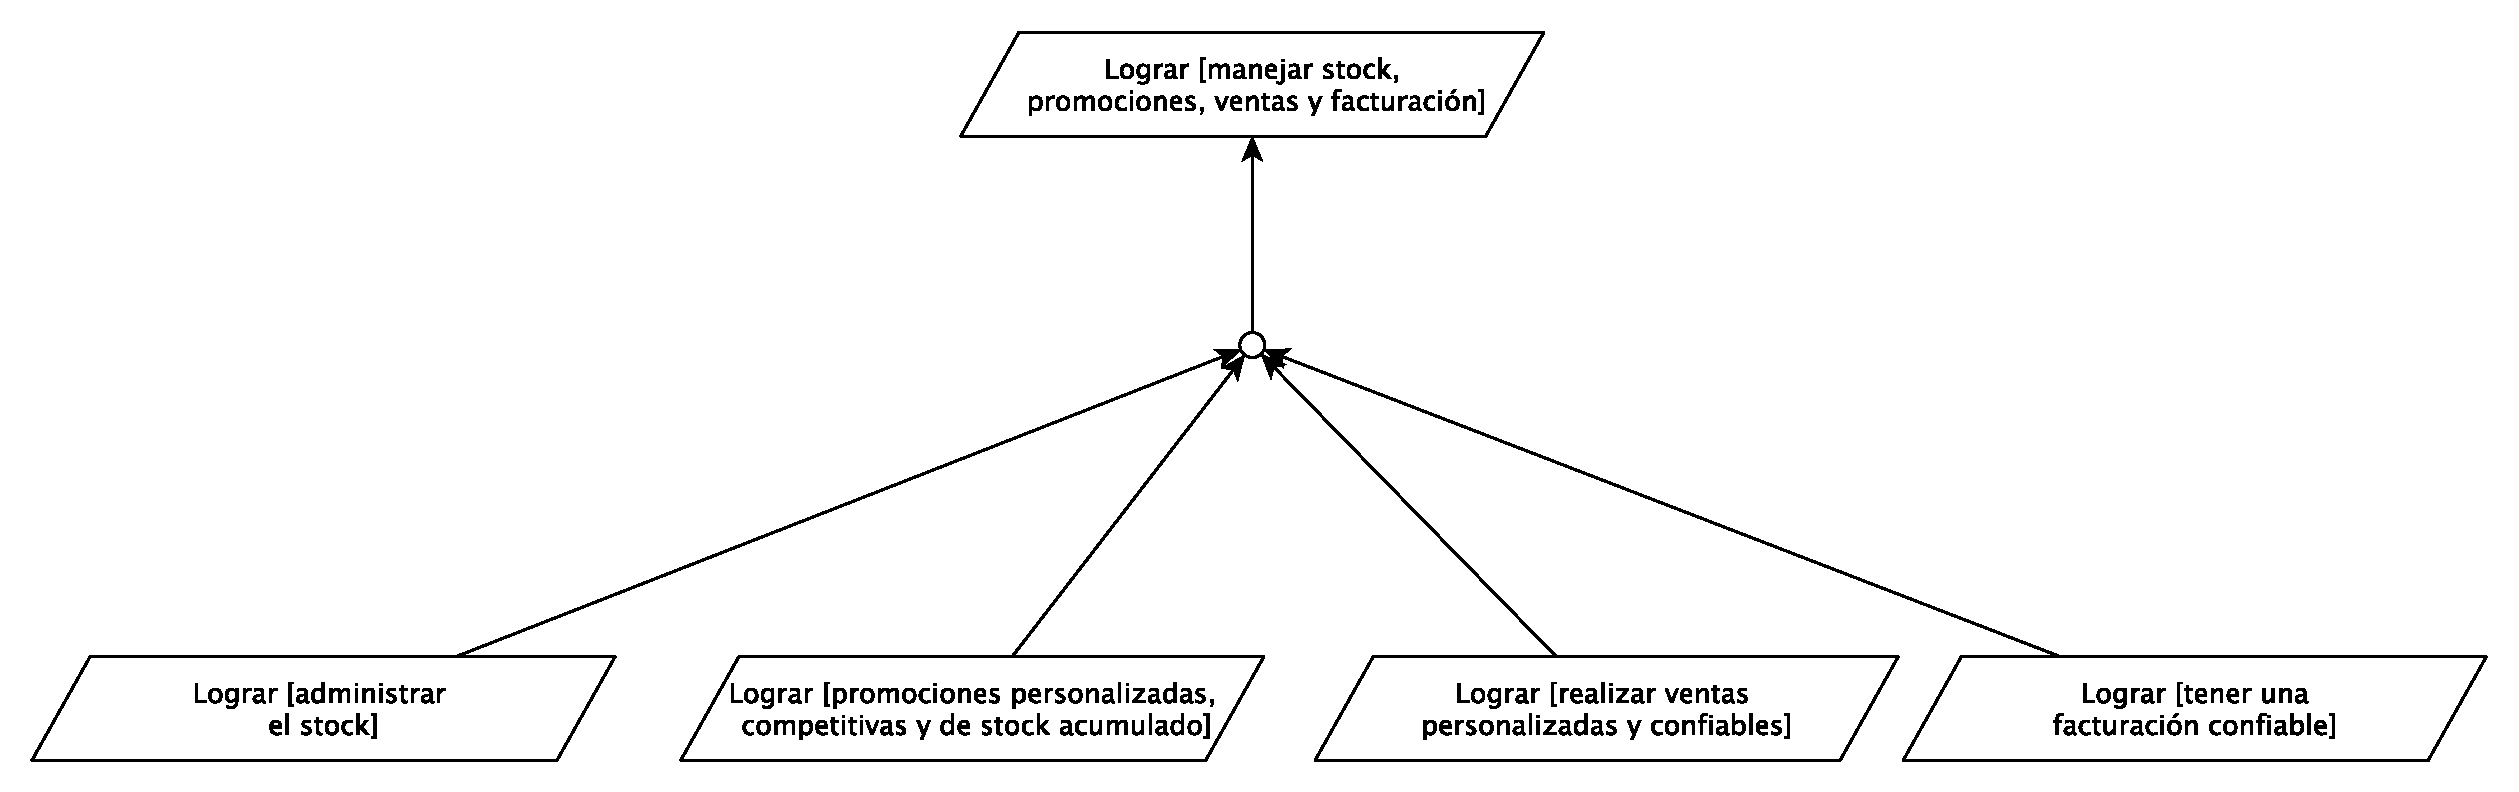
\includegraphics[width=1\textwidth]{./imagenes/general_top.pdf}
  \caption{Diagrama de objetivos - General}
  \label{fig:diagGen}
\end{figure}


\subsection{Rama Stock}

\begin{figure}[h!]
  \centering
  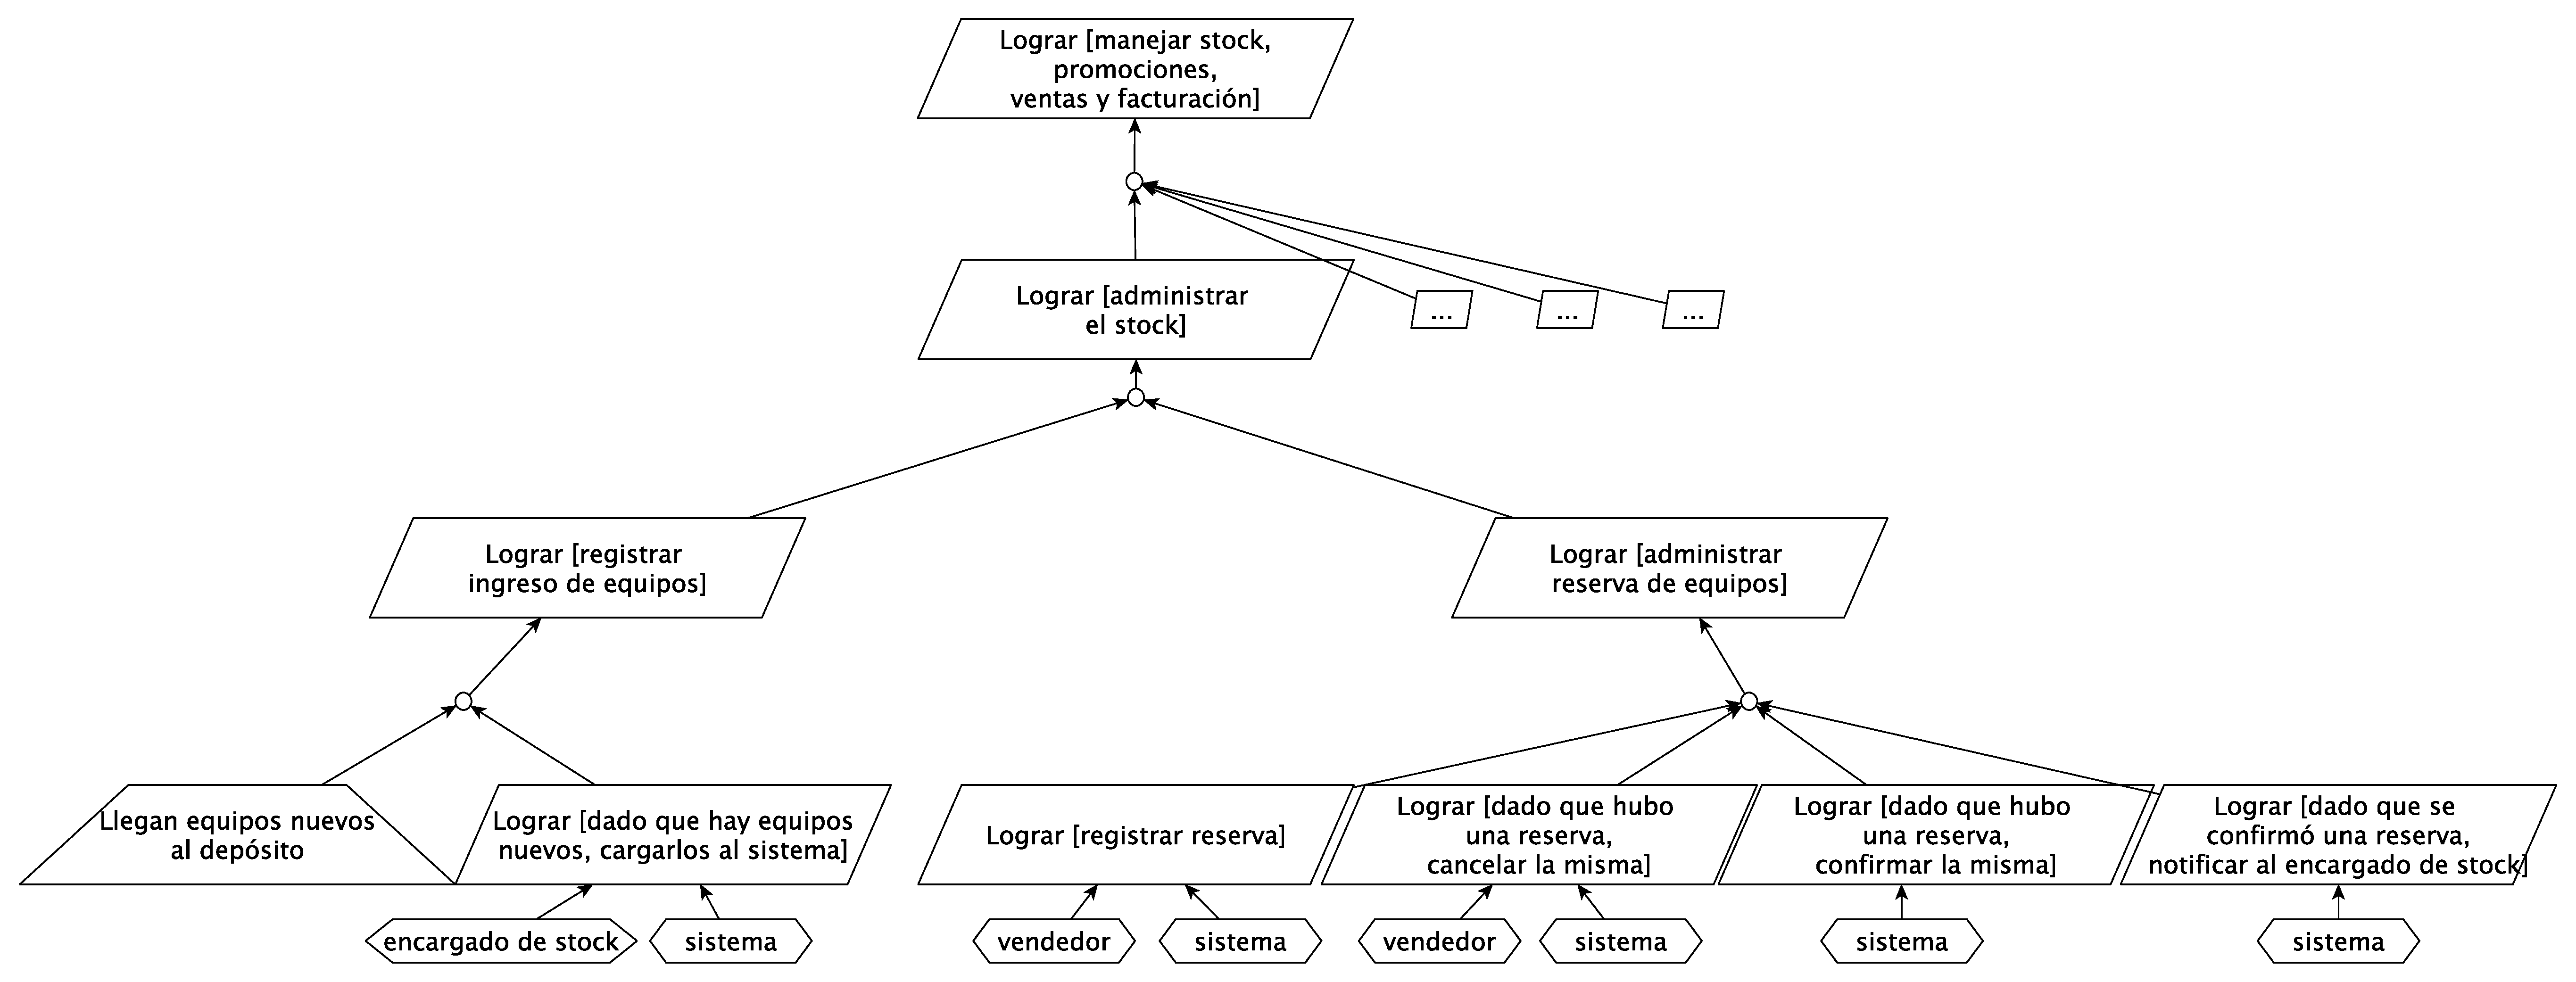
\includegraphics[width=1\textwidth]{./imagenes/stock.pdf}
  \caption{Diagrama de objetivos - Stock}
  \label{fig:diagStock}
\end{figure}

La figura ~\ref{fig:diagStock} presenta la rama de objetivos referente al manejo de stock. La administración del mismo se basa en dos puntos: registrar el ingreso de mercadería nueva y manejar la reserva (y eventual egreso) de los equipos que se vendan. Es importante notar la diferencia entre reserva y venta efectiva (que luego devendrá en egreso del depósito hacia el cliente). Durante la visita del vendedor a un cliente, si éste se decidiera por adquirir una promoción, el vendedor procederá a reservar la misma. Si la reserva le es concedida (ver Rama Ventas), tendrá una ventana de tiempo para confirmar o cancelar la misma. En caso de confirmarla, se le envía una notificación al encargado de stock pero de todas maneras éste deberá aguardar a la notificación de facturación, una vez que la venta haya sido ratificada por el departamento. En caso de cancelación, se restituye la cantidad de stock que se había sacado de circulación al otorgar la reserva para que otros vendedores puedan disponer de esa mercadería. Es importante señalar que la notificación de reserva permite al departamento de stock llevar una cuenta más detallada y controlada del flujo de equipos en sus distintas etapas, a la vez que permite mediante la automatización evitar en un alto grado la disposición errónea de equipos. \\
\indent El control del ingreso de dispositivos móviles es más sencillo y se basa fundamentalmente en la presunción de dominio de que los equipos encargados arriban al depósito en tiempo y forma. Luego, el sistema deberá proveer de una interfaz para que el encargado de stock pueda registrar ese ingreso de manera que esté disponible no sólo para el equipo de ventas sino también para que marketing lance las promociones asociadas con aquellos equipos que sean nuevos y no existieran previamente en el catálogo de la empresa.

\subsubsection{Escenarios}

\begin{itemize}
  \item \textbf{Ingreso de equipos}
    Estéban, el encargado de stock, recibe los nuevos equipos en el depósito y los ingresa en el sistema utilizando la interfaz del mismo.
  \item \textbf{Egreso de equipos}
    Cuando se produce una venta efectiva, el sistema genera una notificación y Estéban debe entregar los equipos al cliente y marcarlos como retirados en el sistema.
\end{itemize}

\subsection{Rama Promociones}

El subárbol de objetivos correspondiente a las promociones fue dividido en dos partes. Satisfacer este aspecto del sistema se basa en cuatro pilares: por un lado lograr promociones parametrizadas y promociones competitivas, objetivos que se exploran en la figura ~\ref{fig:diagProm1}. Por el otro, generar promociones de stock acumulado y mantener actualizado y coherente el catálogo de promociones, metas que se muestran en la figura ~\ref{fig:diagProm2}. En lo que respecta a promociones parametrizadas, este objetivo ataca la necesidad de tener una oferta atractiva para los distintos perfiles de clientes. Gracias a que el sistema lleva cuenta de sus clientes y su historia de consumo, marketing dispone de la información necesaria para crear categorías de clientes en base a la cantidad de líneas que poseen y el dinero que gastan en determinado período y en base a esto generar promociones de acuerdo a los parámetros de estos perfiles. De esta manera, los vendedores podrán optar por consultar promociones a medida del tipo de cliente que visitan de una manera eficiente y rápida.\\
\indent Desde otro enfoque también es importante que las promociones tengan correlación con el estado del mercado y que resulten competitvas respecto de otras empresas de telefonía celular. Para esto deberá conocerse el mercado y luego diseñar ofertas acorde a las conclusiones obtenidas. Aquí se presentan por primera vez alternativas sobre cómo abordar un aspecto del sistema. El alcance del estudio de mercado podrá ser en base a internet o además también en base a los medios de comunicación tradicionales como diarios, revistas, radio, etc. Si bien esta última esfera de comunicación sólo podrá ser analizada manualmente por marketing, una de las alternativas que se ofrece es poder llevar adelante un monitoreo automático de internet (y no manual). A simple vista se puede reflexionar que incorporar al sistema una funcionalidad automática de escaneo del mercado en internet será más costoso y no necesariamente más eficiente que hacerlo de manera manual pero deberá tenerse en cuenta también que permitirá una reacción muy rápida frente a cambios en el mercado para contrarrestar a los competidores. En ese caso, marketing deberá primero definir cierto alcance de la búsqueda como ser sitios, redes sociales, usuarios y canales virtuales de difusión de la empresa. Luego, el sistema procederá a procesar toda esa información y a generar un reporte que será enviado a marketing para su desglose.\\
\indent Una vez que marketing cuenta con el estado de mercado, el objetivo inmediato a satisfacer es la correcta creación de promociones en base a esta información. Nuevamente se ofrecen dos alternativas: la creación manual de las mismas, a cargo de marketing, o una creación automática por parte del sistema pero sujeta a revisión por un agente humano de marketing. Nuevamente la disyuntiva es similar, puesto que incorporar un módulo de creación automáticamente de promociones seguramente será más costoso, pero por otro lado si para el estudio de mercado se decidió realizarlo automáticamente, podría impactar en menor medida en el costo del segundo sistema automático dado que podría procesar de manera eficiente el reporte emitido en el primer paso. Además, con el uso cada vez mayor de las redes sociales e internet para la difusión de promociones y ofertas por parte de las companías, a largo plazo podría resultar muy ventajoso y liberador de recursos humanos contar con autogeneración de promociones competitivas. 
El diseño del sistema no pierde de vista que el objetivo principal de la empresa, en otras palabras, es la rentabilidad. Por eso un objetivo importante que deberá cumplirse es el de la generación de promociones de stock acumulado, es decir, de aquellos conjuntos de equipos que superen cierto número en depósito y sea mejor tratar de despacharlos antes de que se vuelvan obsoletos. Dado que se cumple la administración de stock, el sistema ya cuenta con un monitoreo sumamente actualizado de la mercadería. Según un umbral de alerta definido por el equipo de marketing, el sistema alertará al mismo cuando cierto modele supere ese valor. Otra vez se podrá optar por que marketing diseñe las promociones acordes en este caso de manera manual o que el sistema se encargue y luego marketing las valide. En este caso, la alternativa automatizada no será tan costosa puesto que ya se cuenta con el monitoreo de stock y el tipo de oferta podrá ser parametrizada de antemano por marketing sin mucho problema. De esta manera se ahorrará tiempo y trabajo humano para lograr comercializar de manera efectiva el excedente de mercadería. Por último, es de vital importancia que se pueda regular el catálogo de promociones de manera que se puedan publicar nuevas y no circulen promociones desactualizadas. Todo esto se llevará a cabo mediante una interfaz entre sistema y marketing, lo cual le posibilitará estas acciones al equipo en cuestión. 

\clearpage

\begin{figure}[h!]
  \centering
  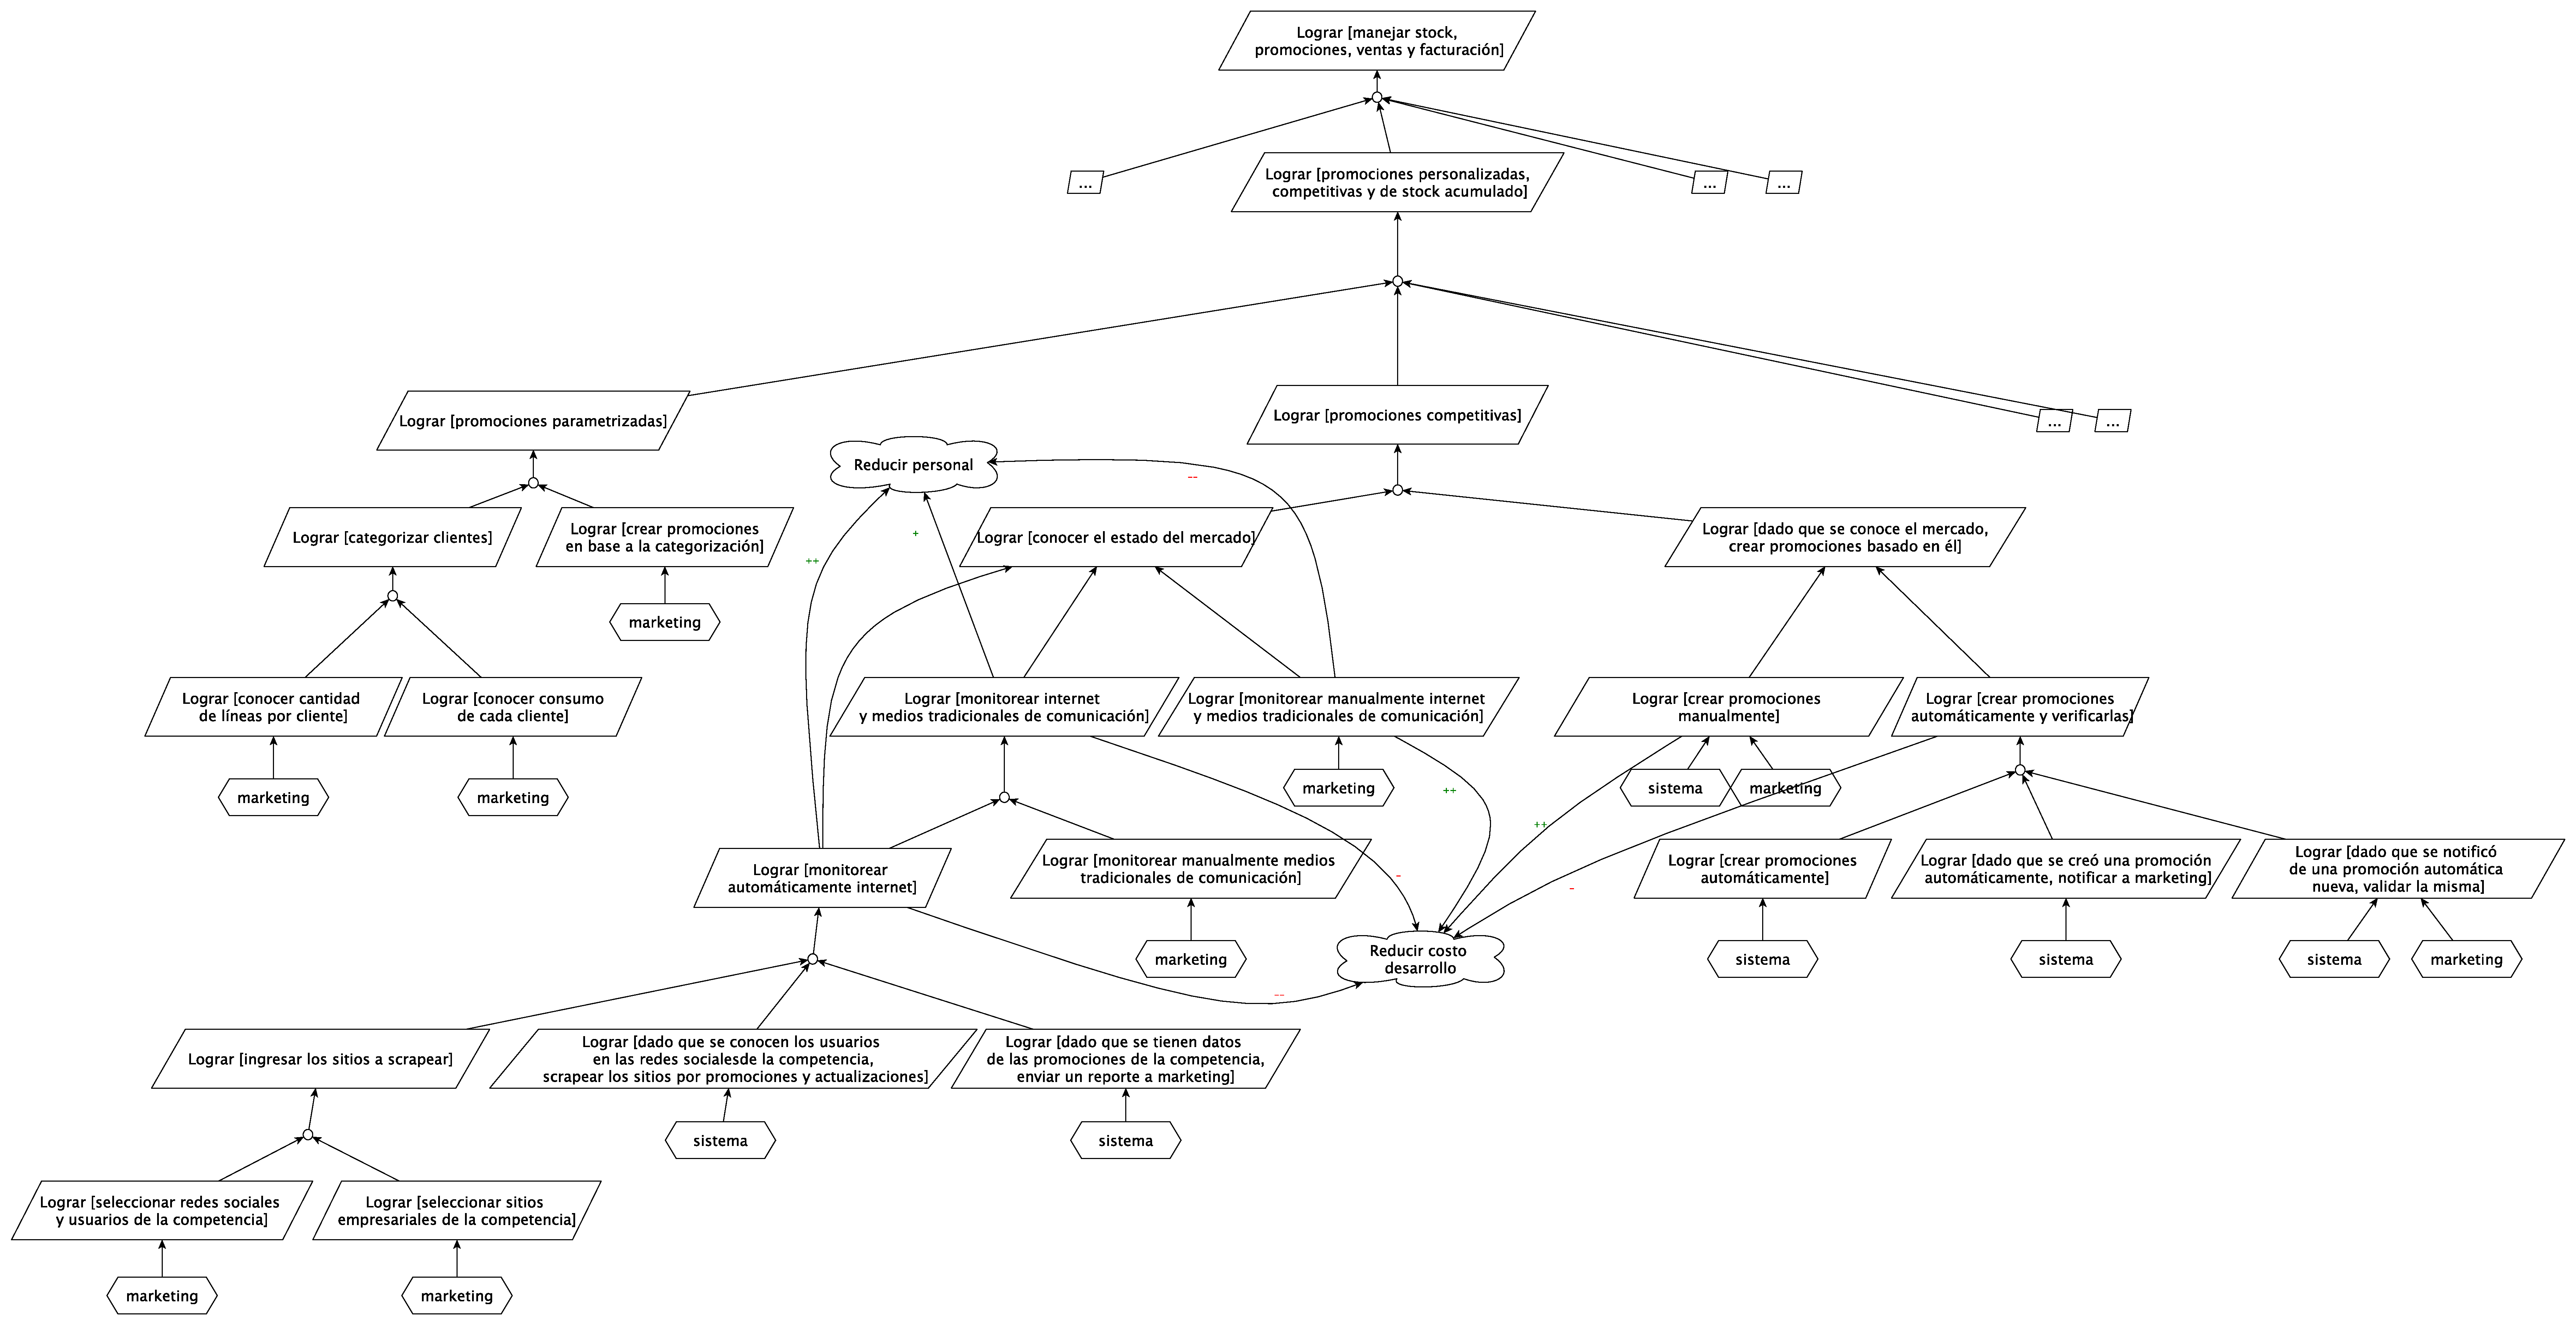
\includegraphics[width=1.5\textwidth, angle=90]{./imagenes/promociones_1.pdf}
  \caption{Diagrama de objetivos - Promociones (parte 1)}
  \label{fig:diagProm1}
\end{figure}

\clearpage


\begin{figure}[h!]
  \centering
  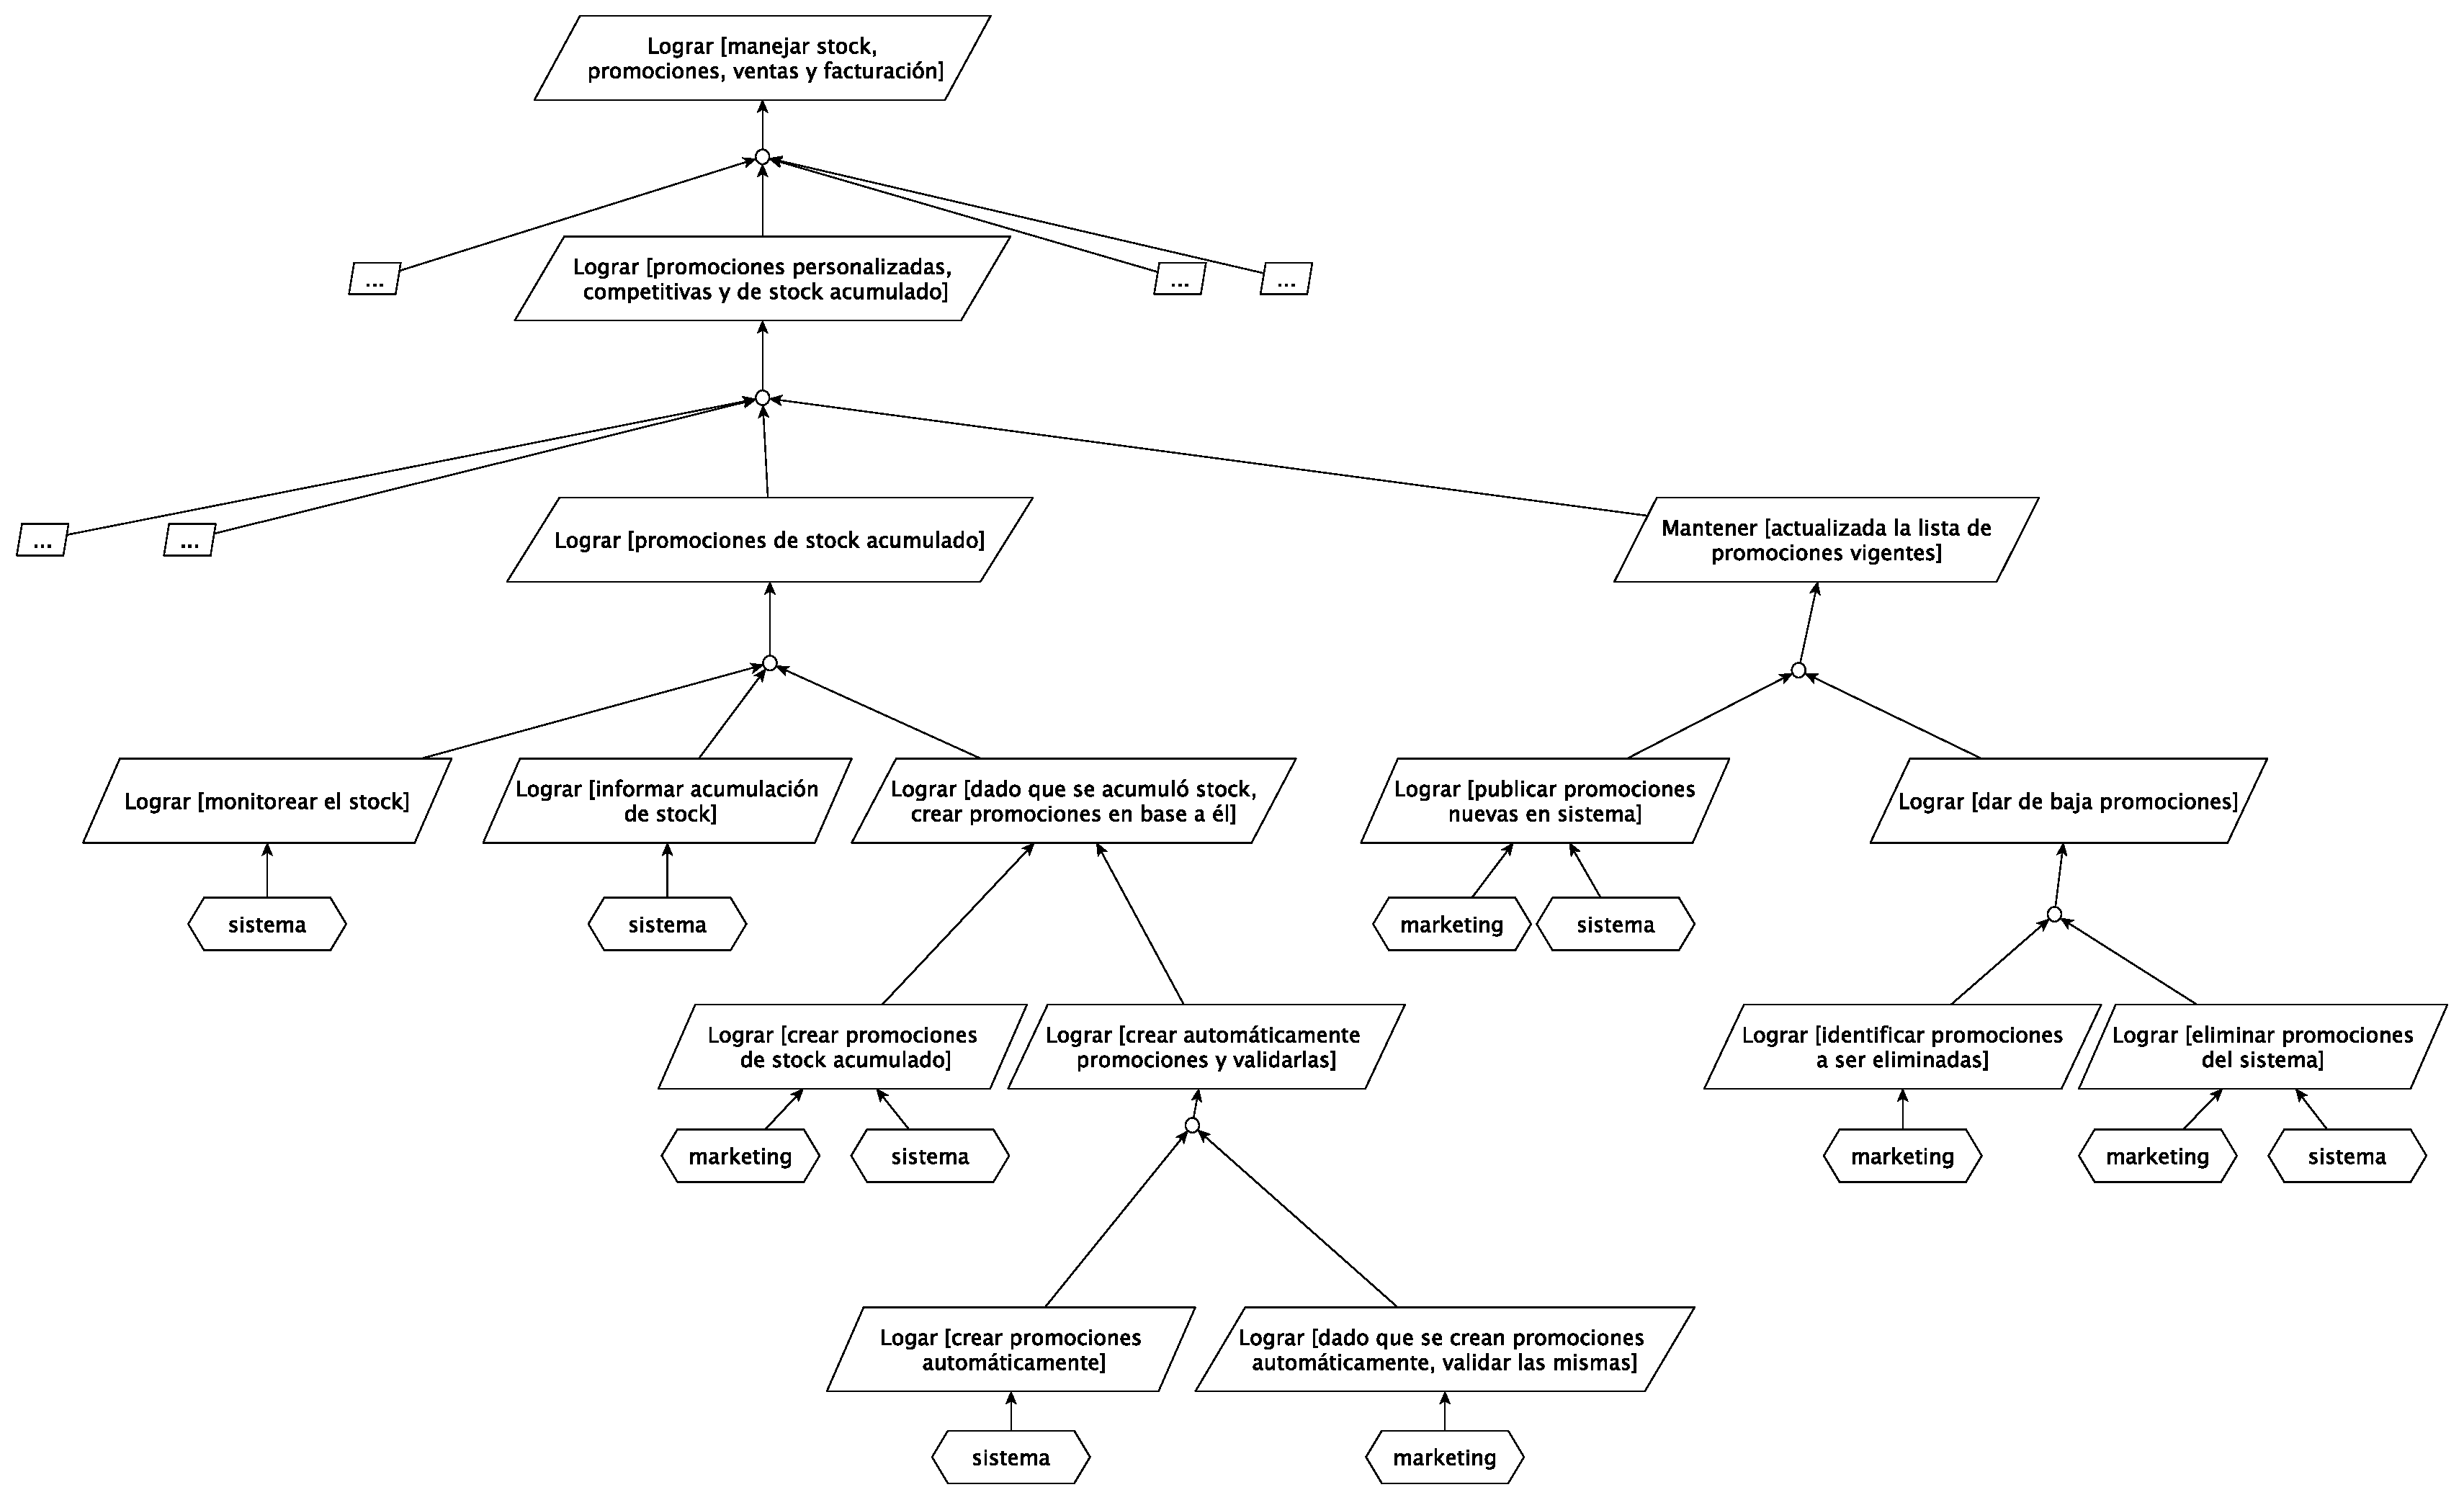
\includegraphics[width=1.3\textwidth, angle=90]{./imagenes/promociones_2.pdf}
  \caption{Diagrama de objetivos - Promociones (parte 2)}
  \label{fig:diagProm2}
\end{figure}

\clearpage

\begin{figure}[h!]
  \centering
  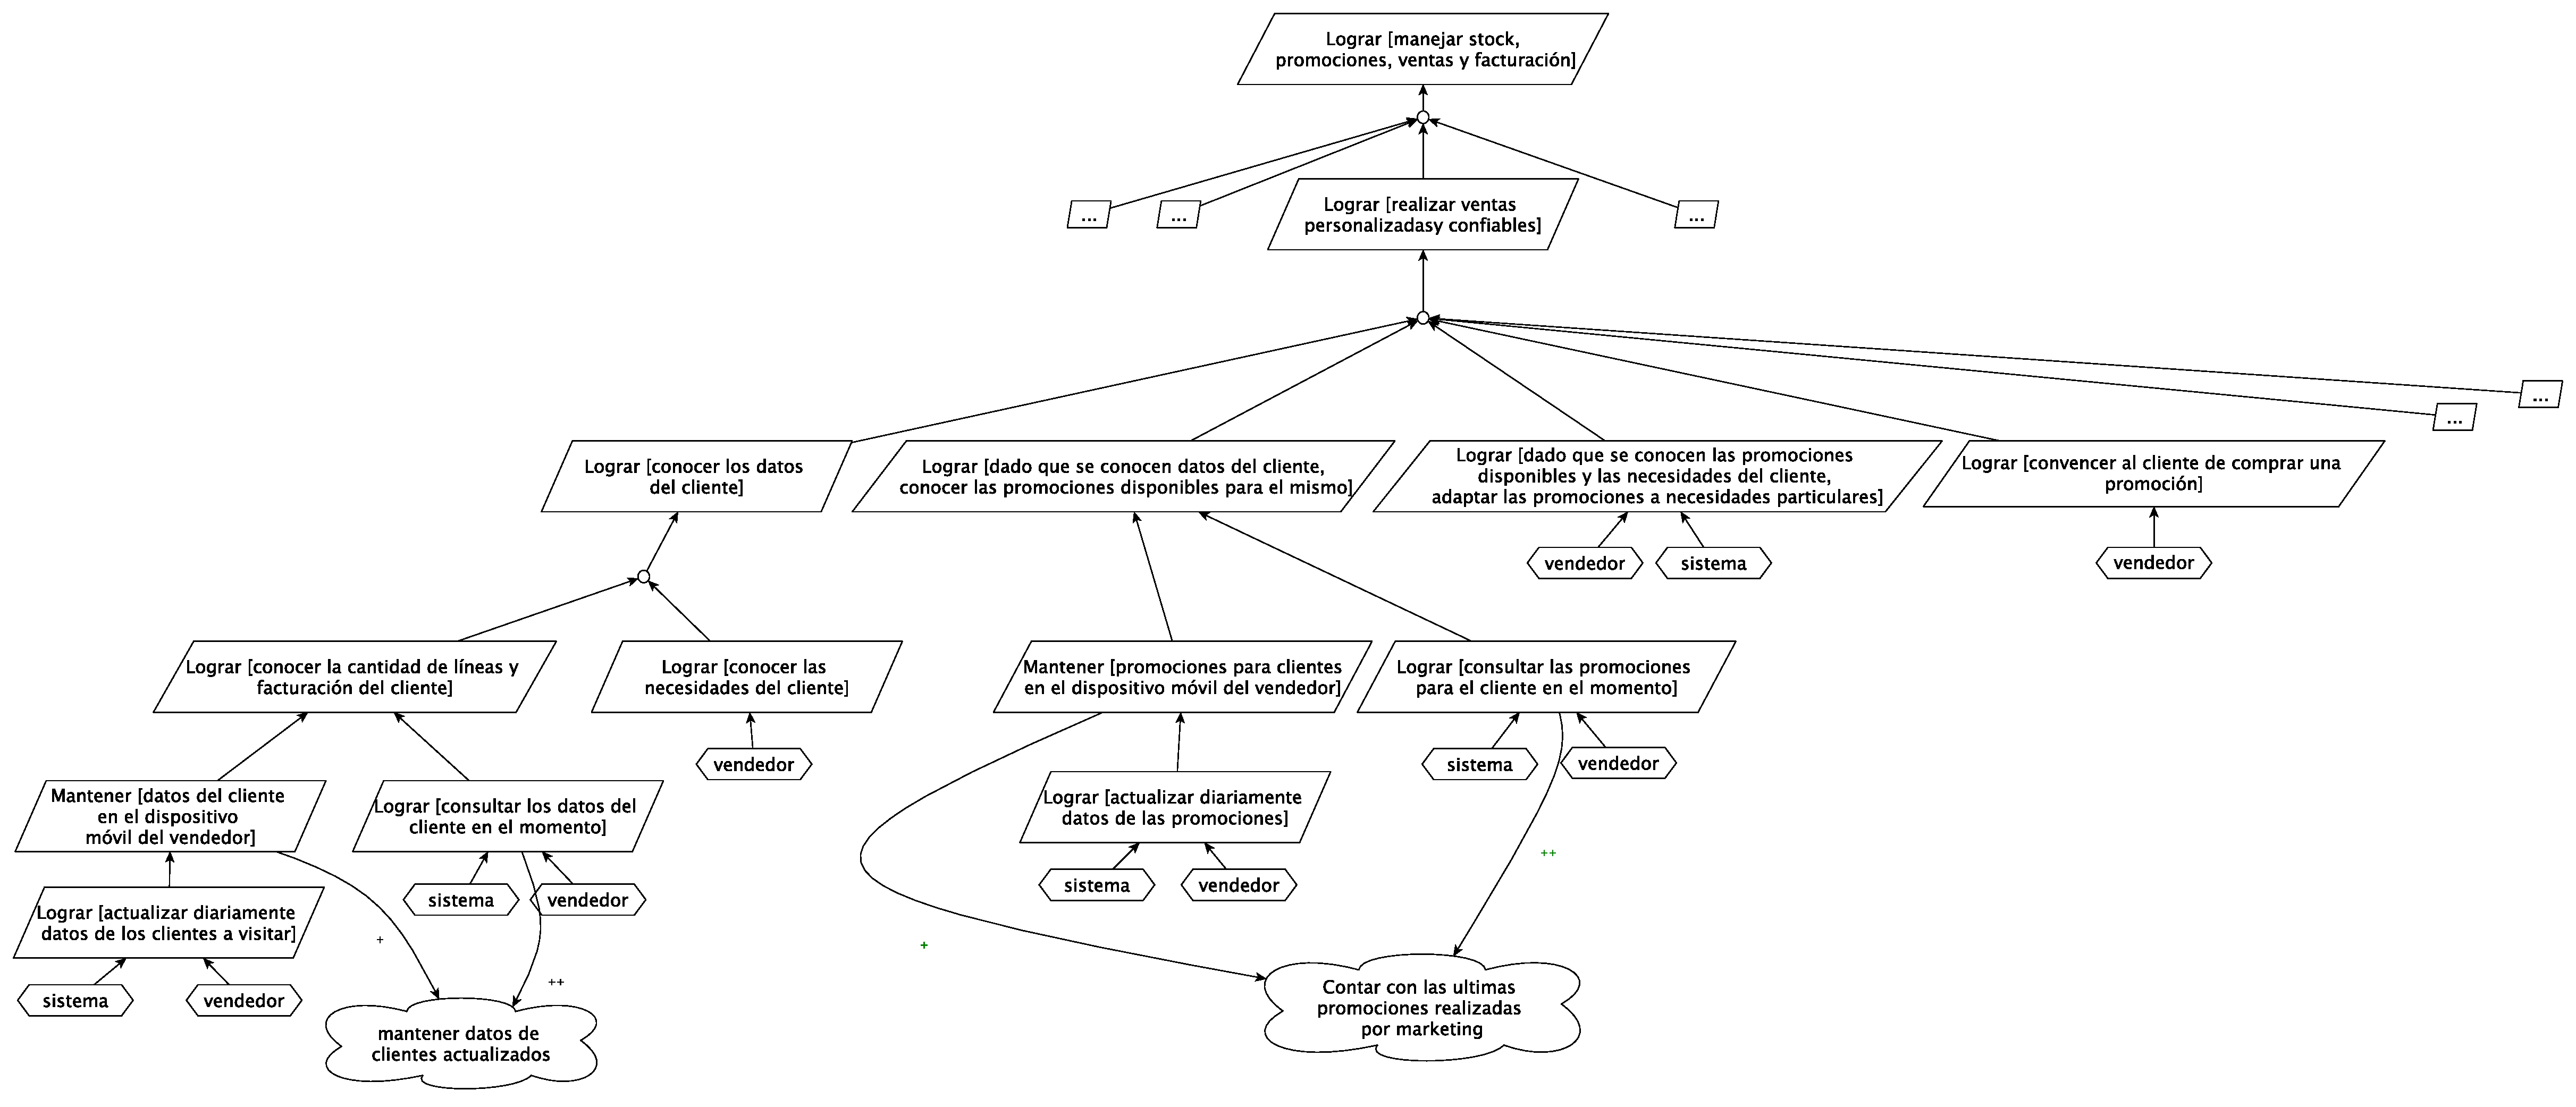
\includegraphics[width=1.5\textwidth, angle=90]{./imagenes/ventas_1.pdf}
  \caption{Diagrama de objetivos - Ventas (parte 1)}
\end{figure}


\clearpage

\clearpage

\begin{figure}[h!]
  \centering
  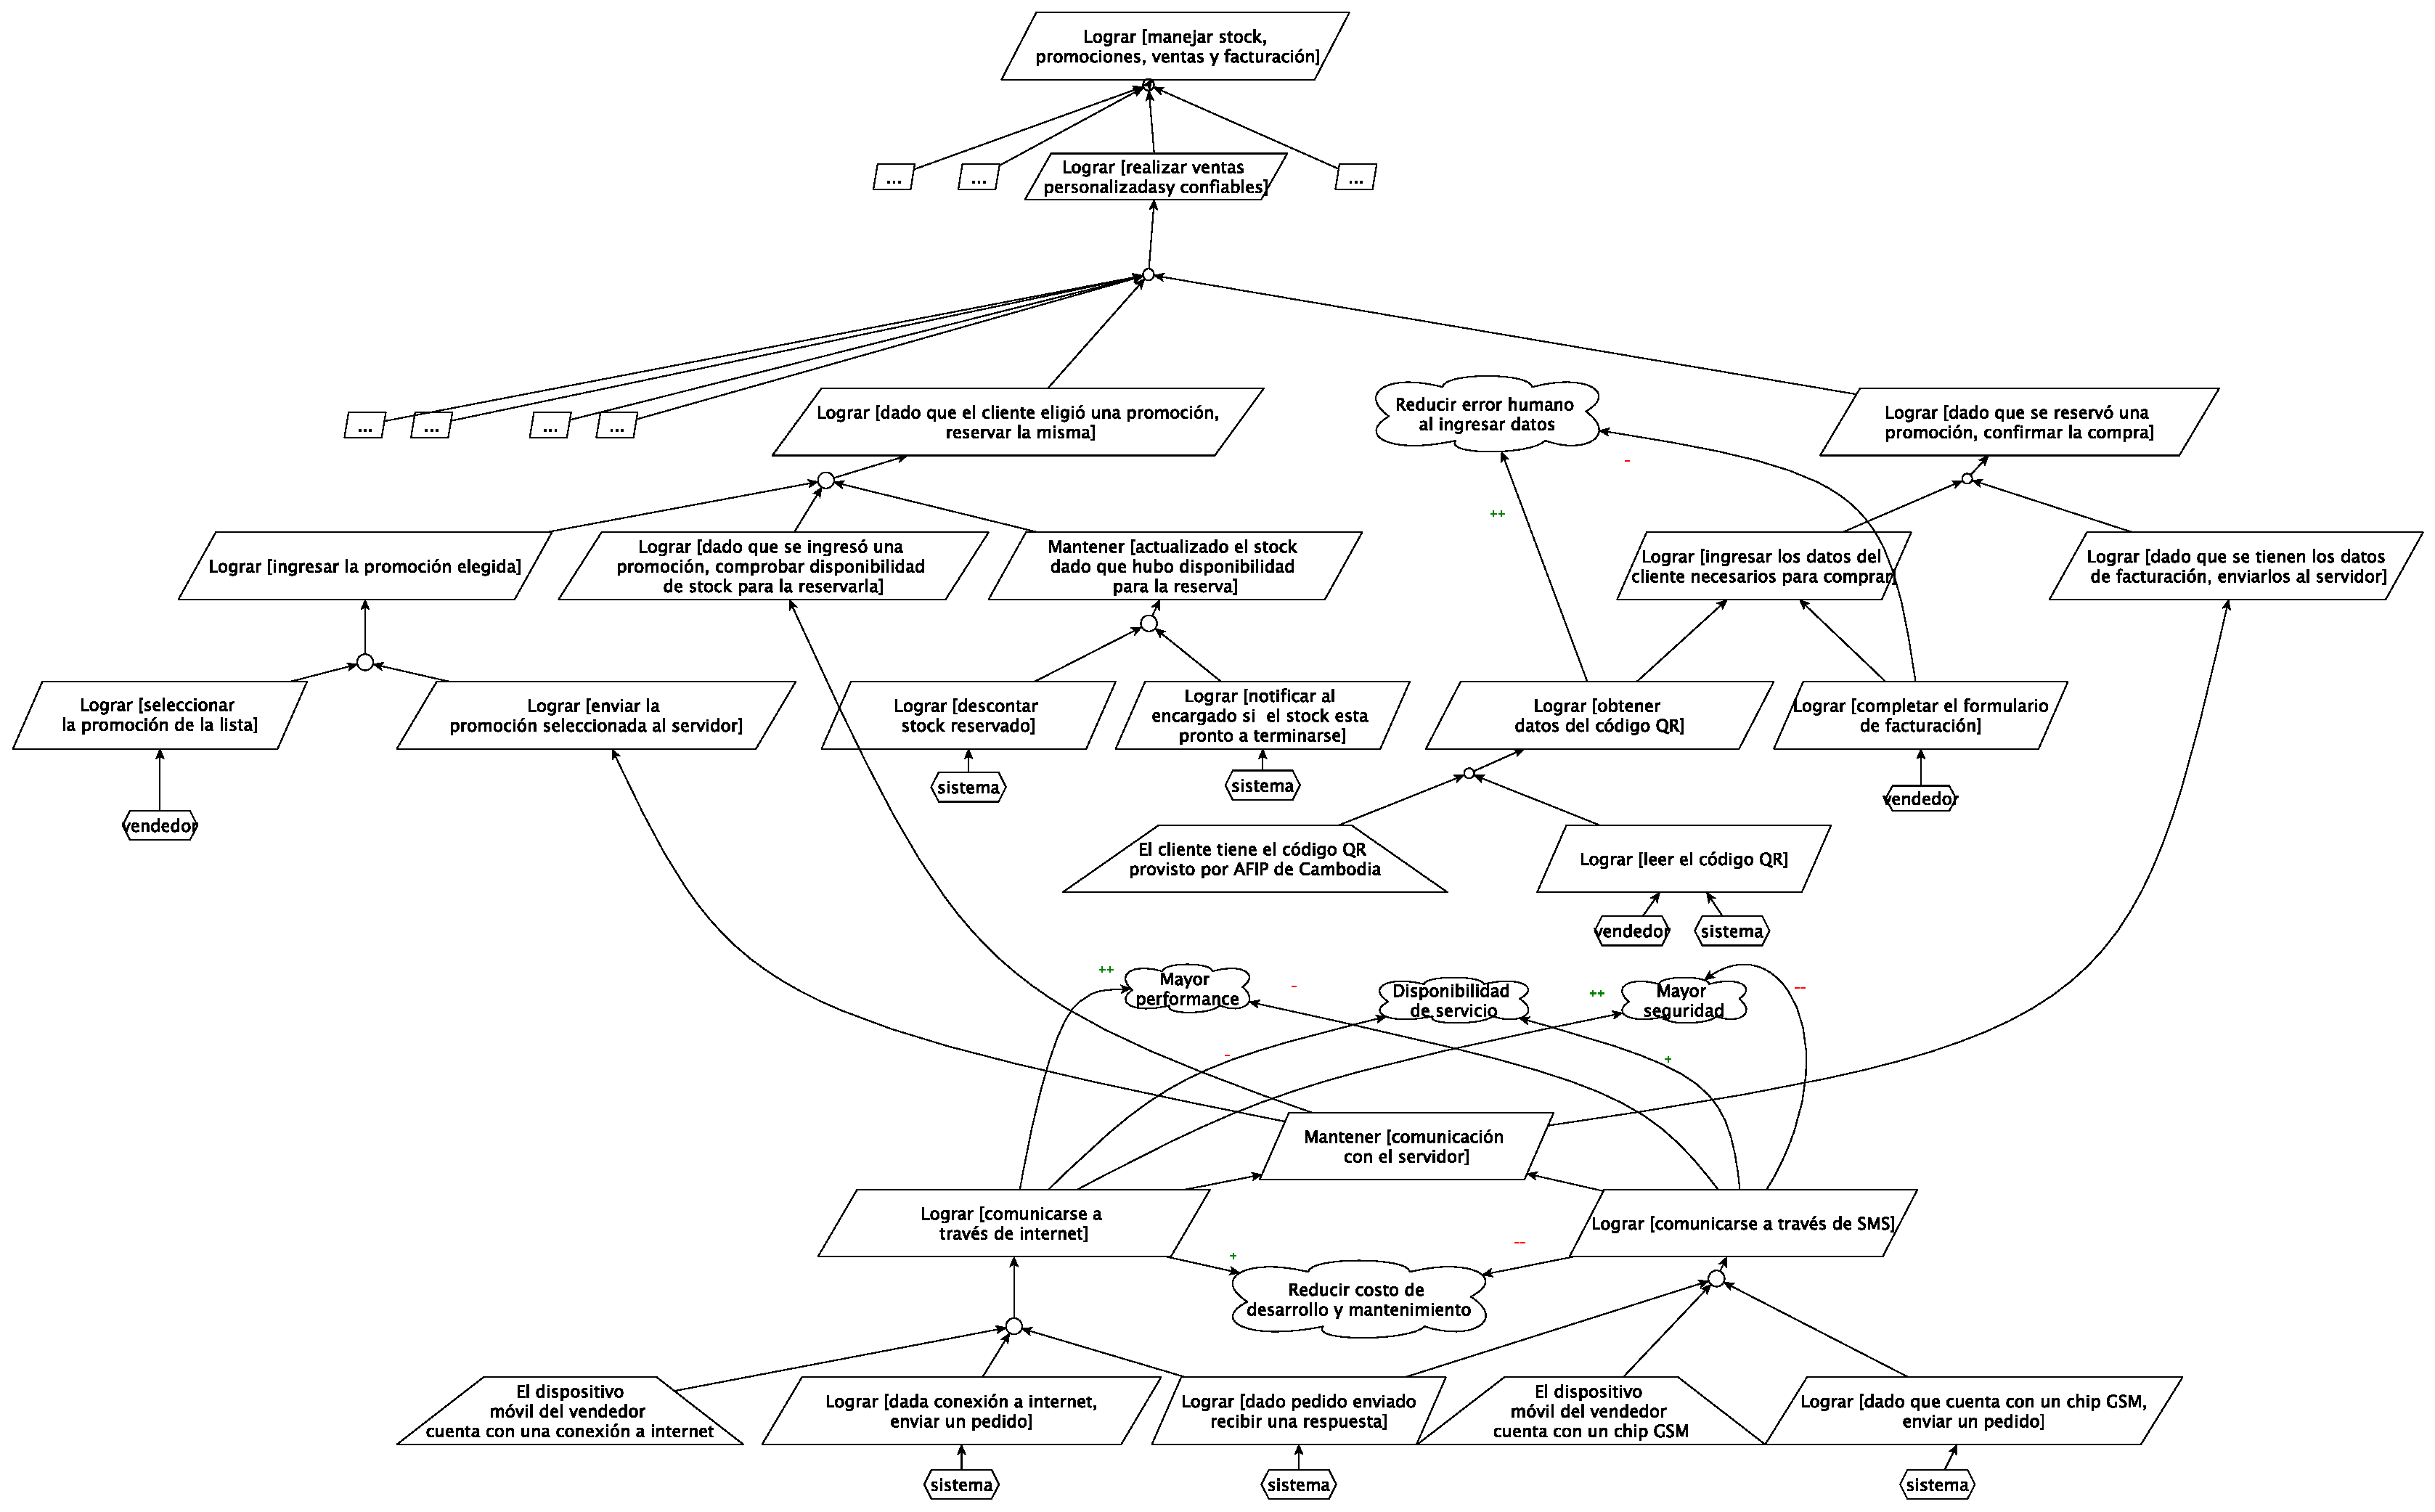
\includegraphics[width=1.5\textwidth, angle=90]{./imagenes/ventas_2.pdf}
  \caption{Diagrama de objetivos - Ventas (parte 2)}
\end{figure}


\clearpage

\begin{figure}[h!]
  \centering
  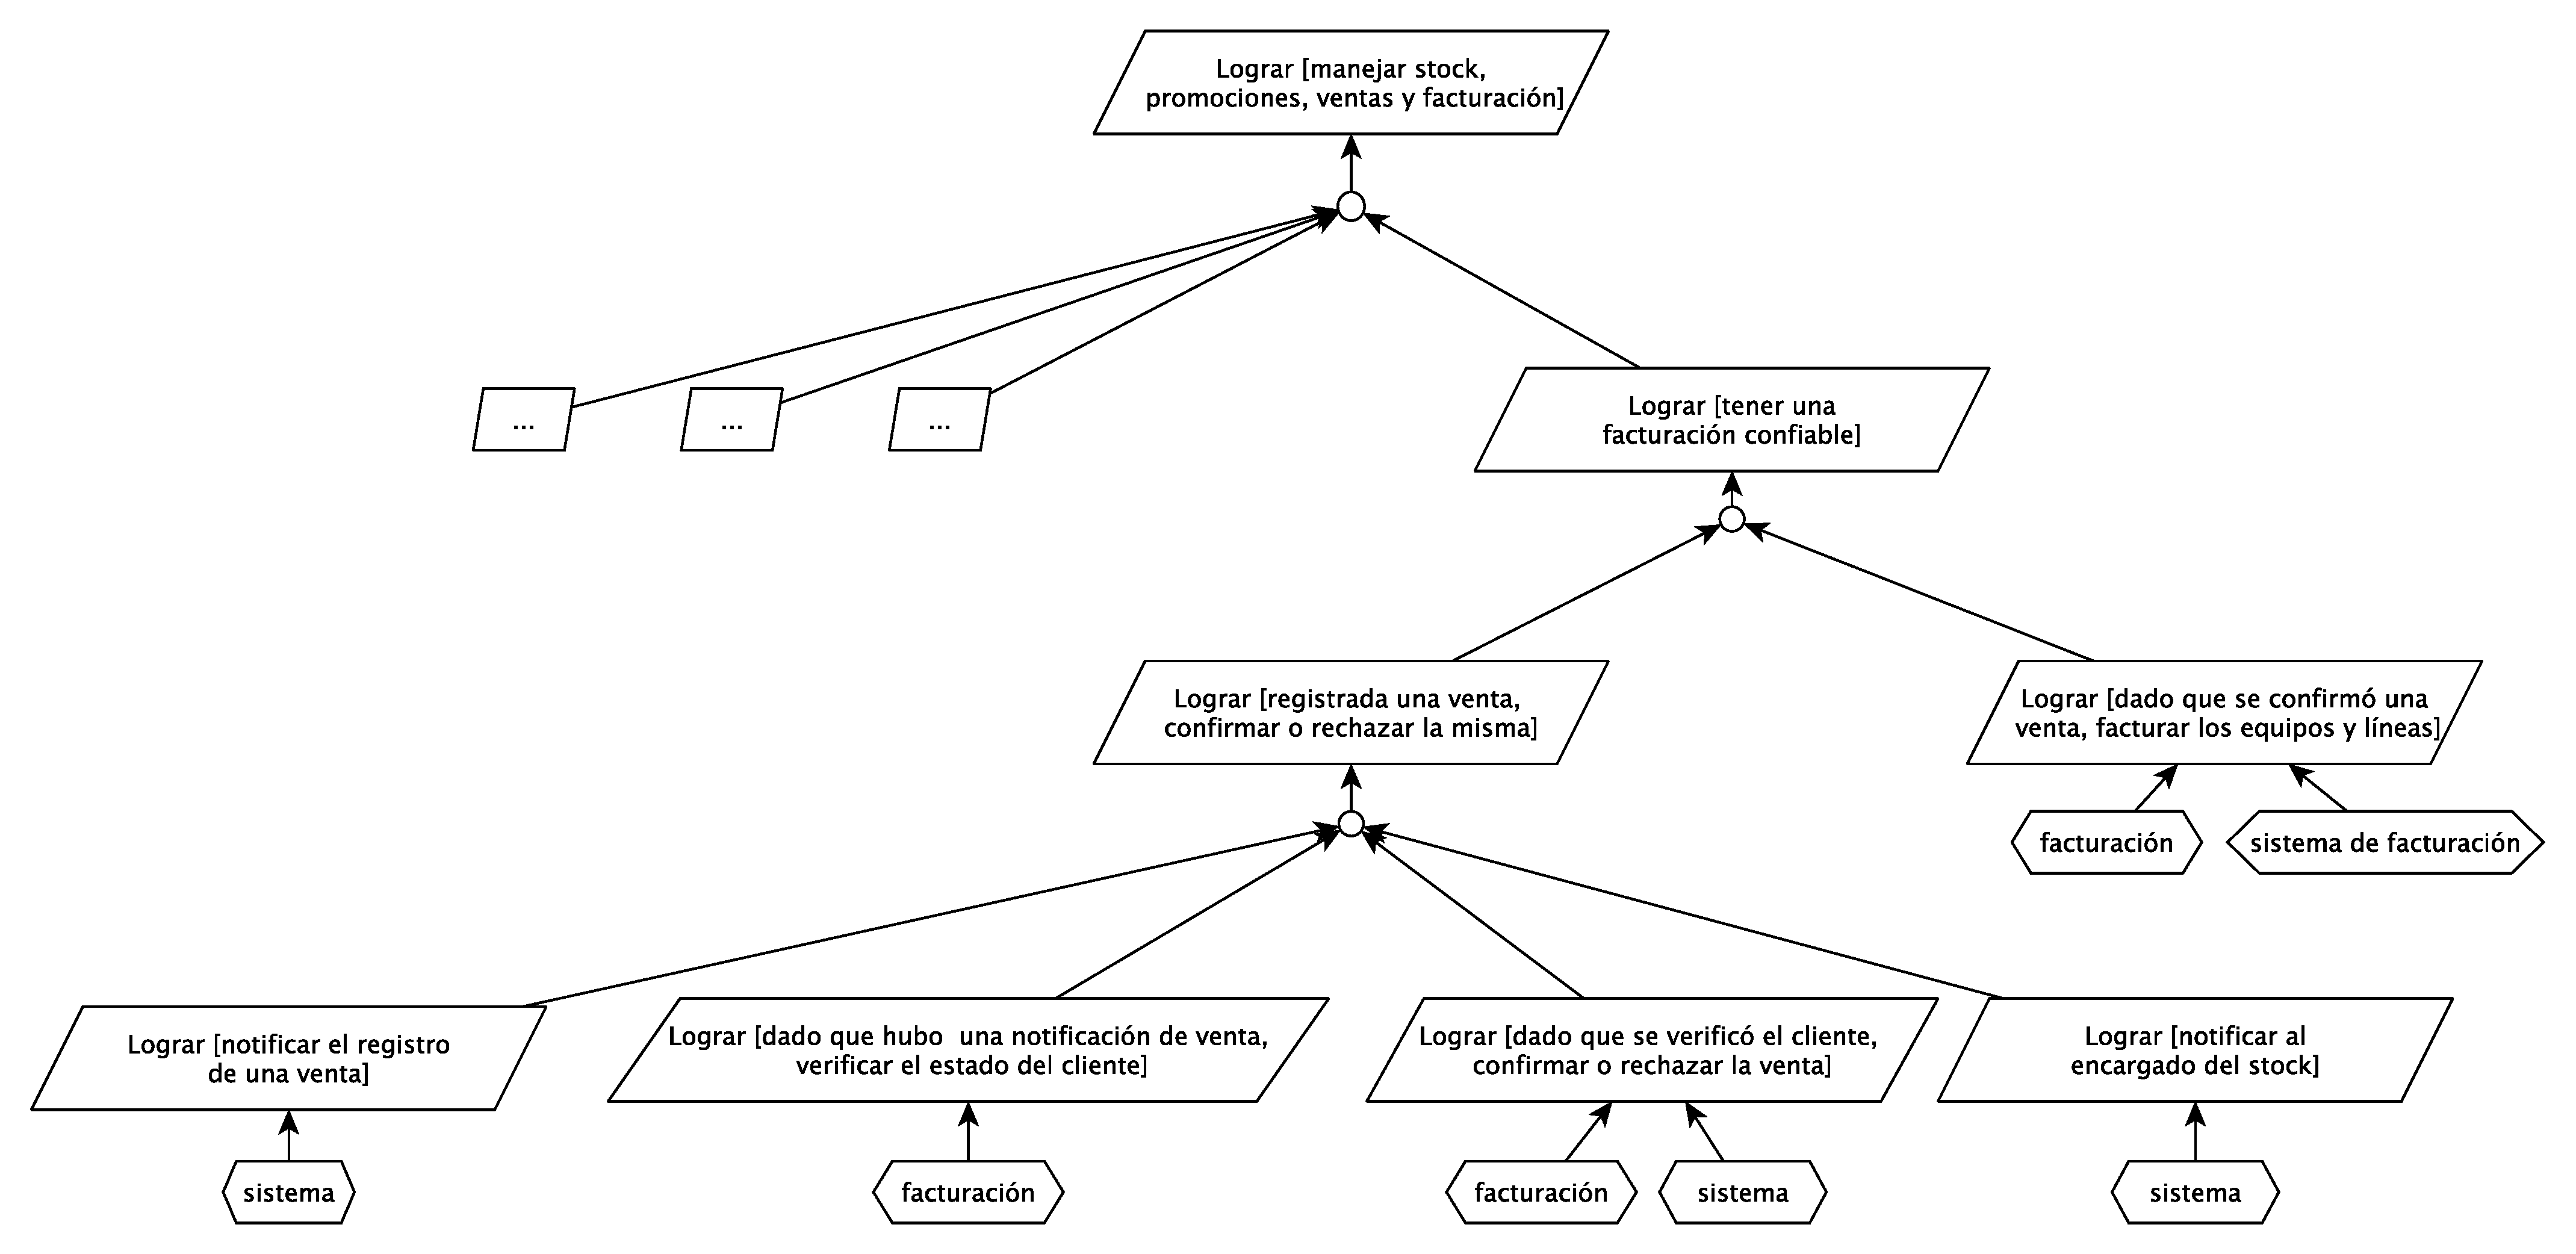
\includegraphics[width=1\textwidth]{./imagenes/facturacion.pdf}
  \caption{Diagrama de objetivos - Facturacion}
\end{figure}

Finalmente, el último pilar sobre el que se apoya la satisfacción del objetivo principal del sistema es el de facturación. En este aspecto se busca una facturación confiable, lo más automatizada posible a partir de las ventas y que no introduzca errores que enlentezcan el proceso de entrega de equipos a los clientes. Para esto, el departamento de facturación recibe la notificación de las ventas realizadas instantáneamente al haber sido realizadas por los vendedores. Luego, deberá proceder a verificar los datos del cliente y chequear que todo esté en regla, lo cual dependerá explícitamente de los estándares de control implementados por el departamento. Una vez que facturación valide al cliente podrá confirmar la venta a través del sistema, lo cual disparará una notificación al encargado de stock para que se ocupe de armar y coordinar la entrega. Por otro lado, facturación deberá seguir más allá y, utilizando los datos digitalmente provistos por el sistema de ventas, realizar la facturación correspondiente en su sistema externo para tal fin. De cualquier manera se garantizará que haya compatibilidad entre ambos sistemas con el objetivo de que los empleados de facturación no necesiten reingresar ningún dato de manera manual y así poder reducir posibles errores en la etapa final del proceso.

